%!TEX root = ../Thesis.tex
\chapter{Cases}\label{cha:cases}
This chapter introduces the different cases this thesis looks into. 

\section{Pelton needles}\label{sub:pelton_needles}

    \begin{itemize}
        \item Explore the possibility to detect the anomalies/novelties connected to the reported control problems with the pelton needles, by using only the process signals from the needles  
        % \item Discuss the issue with uneven sample frequency for different signals, mention different techniques for interpolation of missing data, is this a good option? why or why not? 
        \item Look at different methods for unsupervised feature selection. The datasets holds many signals, which ones can hold vital information for the needle control problem? 
        \item Look at different methods for supervised feature selection, using the RMSE between the pairwise needles as a target variable. 
        \item Analyze the features selected in the two different techniques, are they similar? If not, what seems to be the main difference between the two techniques? 
        \item use principal component analysis (PCA) and kernel PCA to reduce the number of features by linear an non linear combinations of the original feature set. Create a reduced data-matrix based on the principal components which again can be used as input for the machine learning algorithms. 
        \item Look into anomaly/novelty detection comparing the performance of different algorithms, on the different feature sets. The following list is a suggestion to algorithms, at least two should be used. Compare the algorithms in regards of performance, complexity, run-time, etc. 
        \begin{itemize}
            \item One class support vector machine
            \item Density based anomaly detection, k-nearest neighbors
            \item Clustering based anomaly detection, k-means clustering 
            \item Neural Networks 
        \end{itemize}
        \item Explain necessary steps to enable the use of the techniques in power plants, what are the challenges? What needs to be overcome before the results can be incorporated into any power plant using pelton turbines?     
        
    \end{itemize}
    
    As mentioned, there was data available from two different power plants with pelton turbines controlled in a similar maner. One of plants had recorded several issues with the needle control, and was used as a case to test early detection of problems with the needle operation. 
    
    \begin{figure}
        \centering
        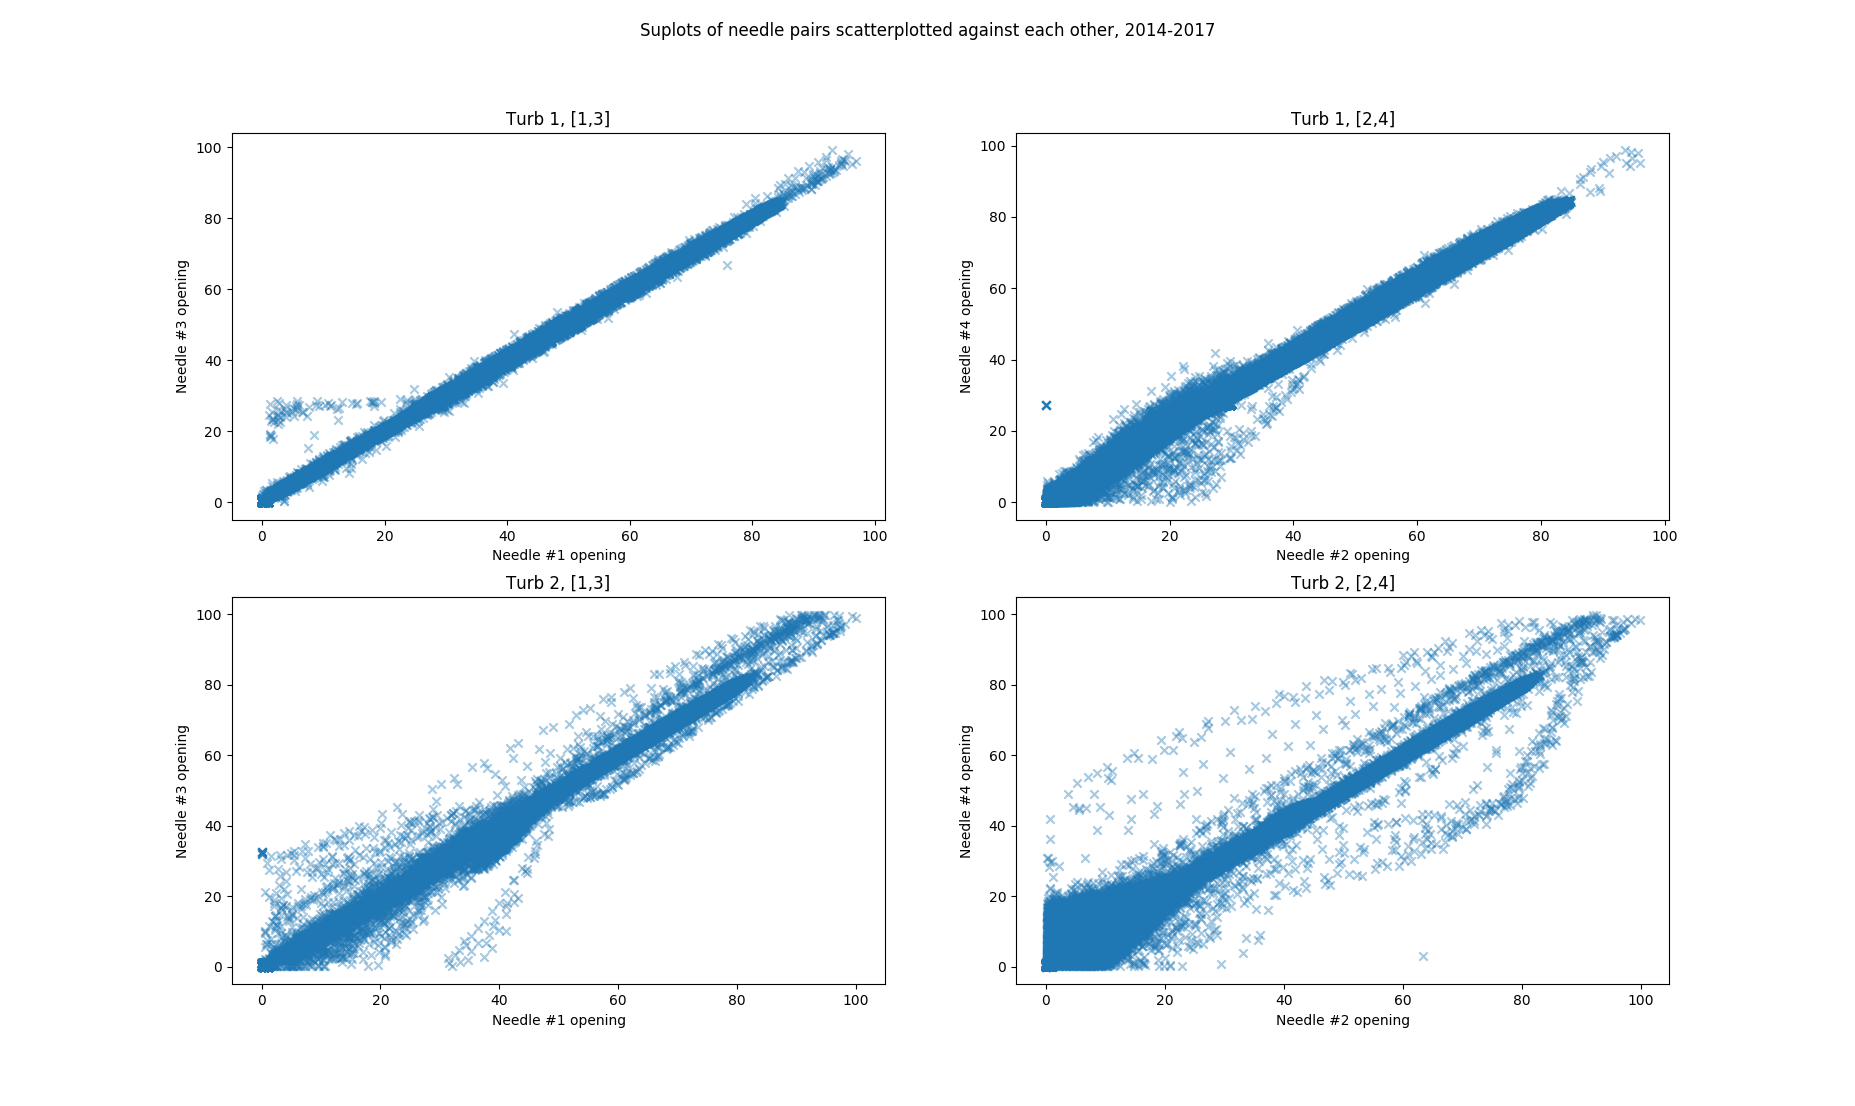
\includegraphics[width=\textwidth]{report/figures/analysis/hjartdola/hjar_scatterplot_all_needels.png}
        \caption{Caption}
        \label{fig:my_label}
    \end{figure}
    
    
    \begin{figure}
        \centering
        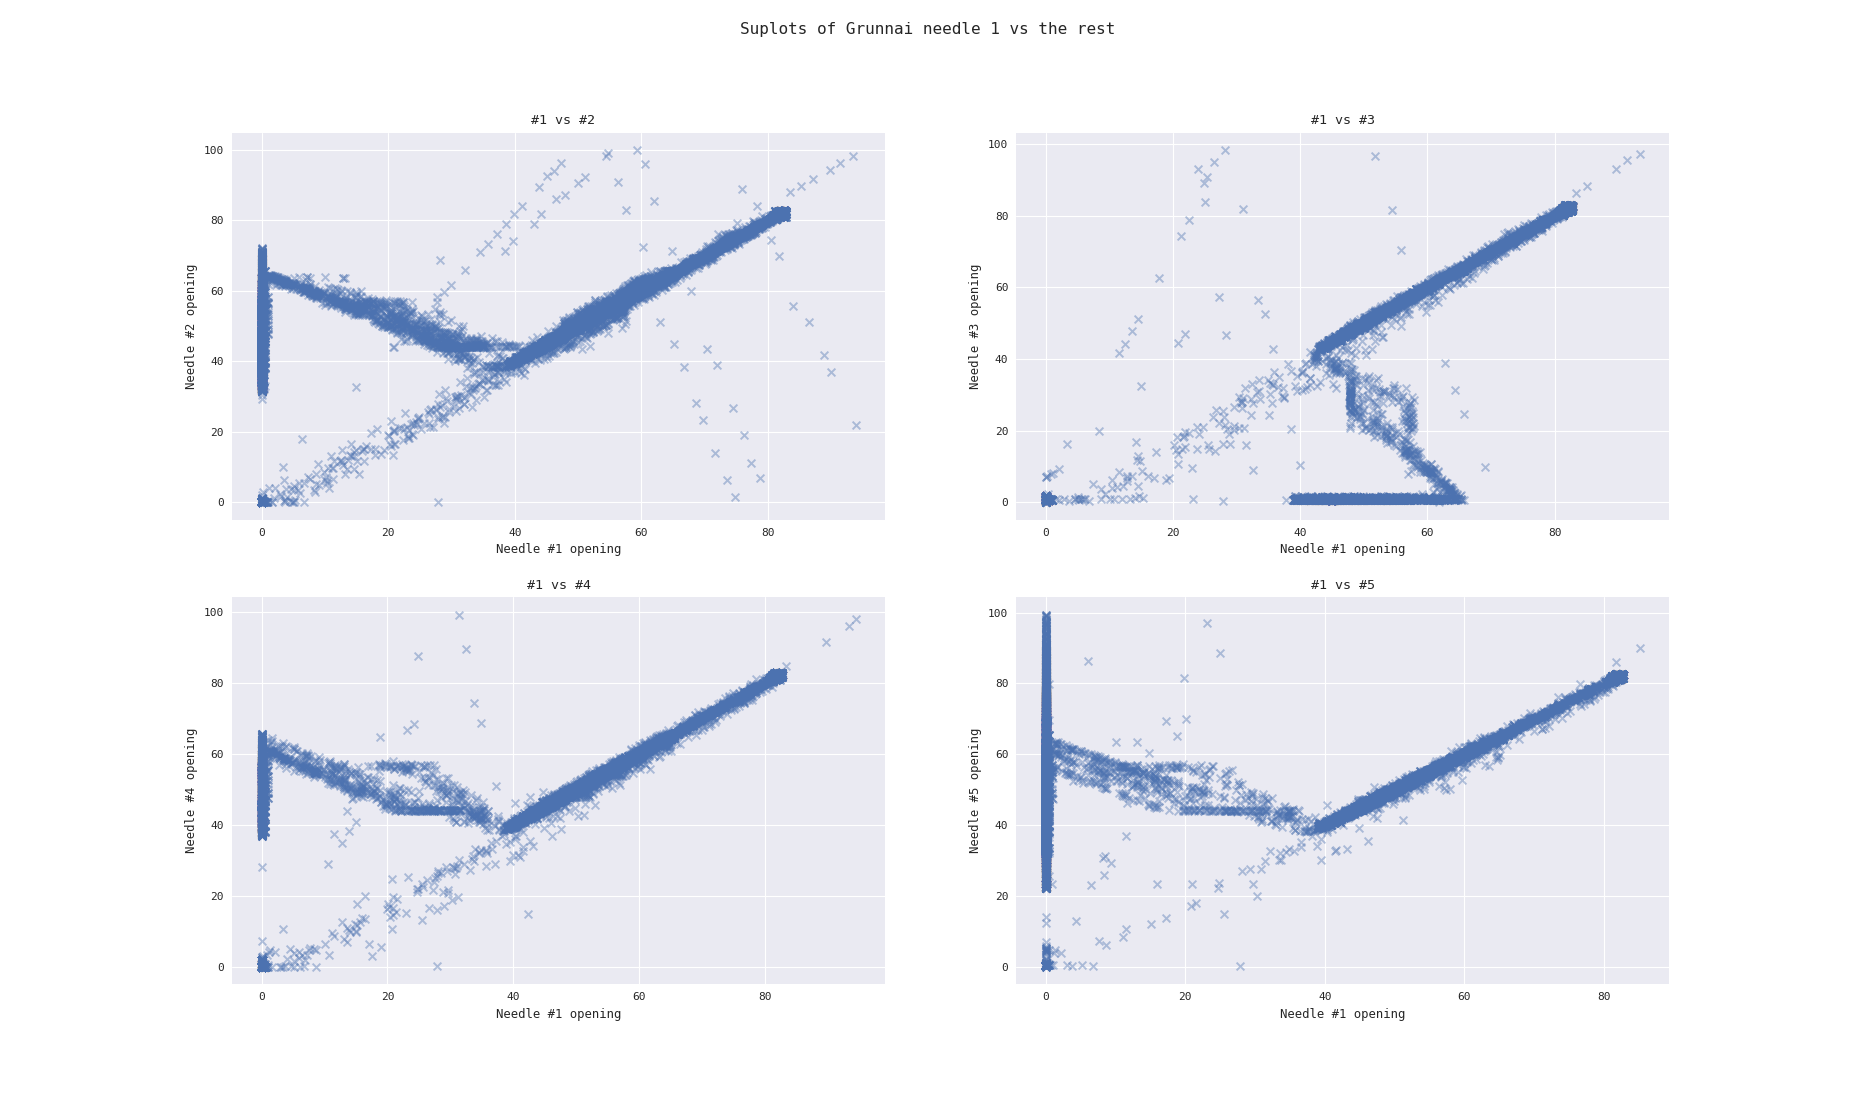
\includegraphics[width=\textwidth]{report/figures/analysis/grunnai/grun_scatterplot_1_vs_rest.png}
        \caption{Caption}
        \label{fig:my_label}
    \end{figure}
    
    
    \begin{figure}
        \centering
        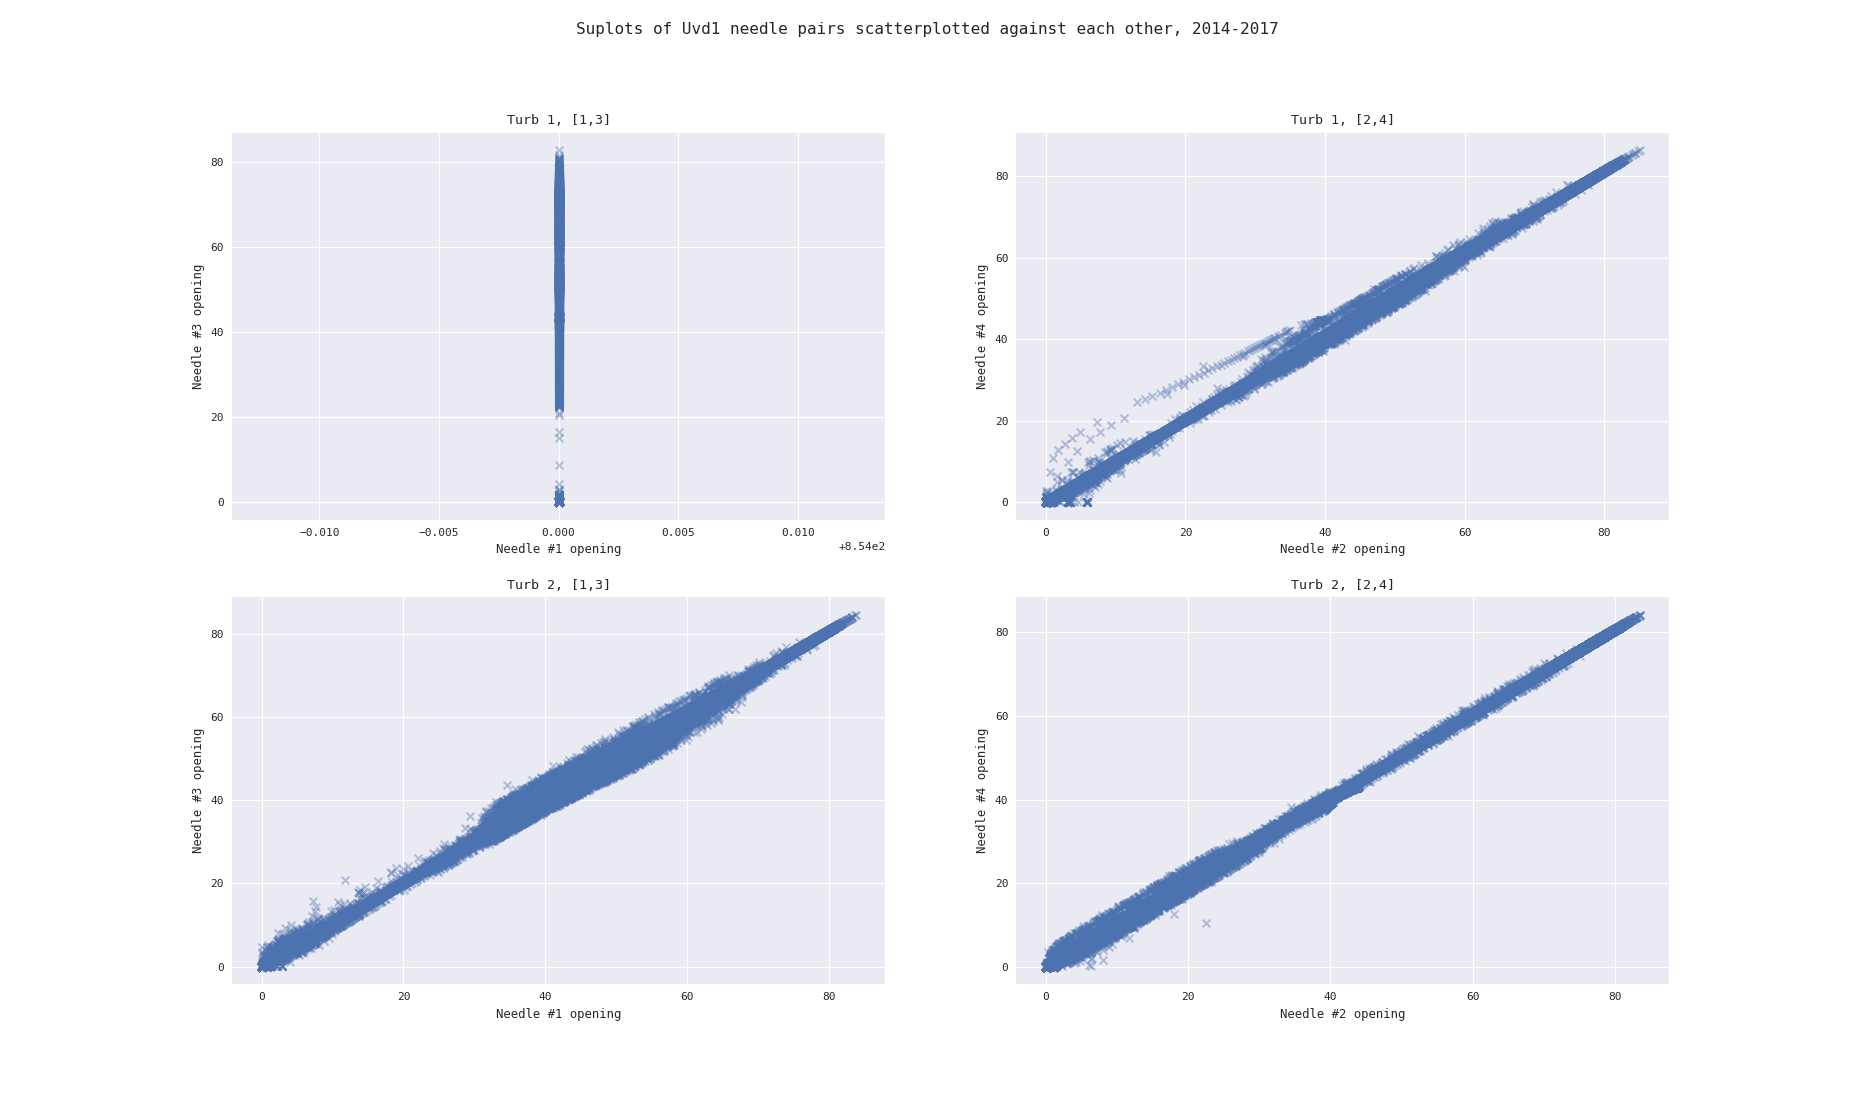
\includegraphics[width=\textwidth]{report/figures/analysis/uvdal1/uvd1_scatterplot_all_needels.png}
        \caption{Caption}
        \label{fig:my_label}
    \end{figure}
    
    
    
    It is important to understand that an outlier in the data does not necessarily mean that something is about to break. There is a possibility that the sample is an indication of a condition change in the equipmnet, but it might also be due to error in the measurement, noise or just a deviation in the ongoing process. This makes this kind of analysis even harder, an outlier might just be a coincident, that yields little to no information. 
    
    The following quote from \cite{Malhotra2016} is an example of issues one need to handle in the following analysis. "In real-world sensor data from machines, there are scenarios when the behavior of a machine changes based on usage and external factors which are difficult to capture" \todo{flytte? Bra sista men kanskje litt malplassert?}
